%!TEX program = pdflatex
% Target: Journal of Physics A: Mathematical and Theoretical, regular paper.
% Drafted in REVTeX with the IOP bibliography style; converts to the
% publisher's class on acceptance.
\documentclass[
  aps,pre,
  reprint,
  superscriptaddress,
  amsmath,amssymb,
  floatfix
]{revtex4-2}

\usepackage{graphicx}
\usepackage{bm}
\usepackage{xcolor}
\usepackage{hyperref}
\hypersetup{colorlinks=true,
            linkcolor=blue!55!black,
            citecolor=blue!55!black,
            urlcolor=blue!55!black}
\usepackage{amsthm}
\usepackage[capitalize,nameinlink]{cleveref}

\theoremstyle{plain}
\newtheorem{theorem}{Theorem}
\newtheorem{lemma}[theorem]{Lemma}
\newtheorem{proposition}[theorem]{Proposition}
\newtheorem{corollary}[theorem]{Corollary}
\newtheorem{conjecture}[theorem]{Conjecture}

\theoremstyle{definition}
\newtheorem{definition}[theorem]{Definition}
\newtheorem{example}[theorem]{Example}

\theoremstyle{remark}
\newtheorem{remark}[theorem]{Remark}

\newcommand{\BFC}{1\text{-}\mathbb{BFC}^{(r)}_2}
\newcommand{\BFCm}{1\text{-}\mathbb{BFC}^{(m)}_2}
\newcommand{\BFCthree}{1\text{-}\mathbb{BFC}^{(3)}_2}
\newcommand{\Fld}{\mathbb{F}}
\newcommand{\Disc}{\mathcal{D}}
\DeclareMathOperator{\rank}{rank}

\begin{document}

\title{Boundary $K$-matrices at every Fuss--Catalan rank}

\author{Zhiyuan Yao}
\email{yaozy@lzu.edu.cn}
\affiliation{Lanzhou Center for Theoretical Physics, Key Laboratory of Theoretical Physics of Gansu Province, Key Laboratory of Quantum Theory and Applications of MoE, Gansu Provincial Research Center for Basic Disciplines of Quantum Physics, Lanzhou University, Lanzhou 730000, China}

\date{\today}

\begin{abstract}
The Fuss--Catalan algebras replace each site of a Temperley--Lieb chain by a
bundle of $r$ nested coloured strands, and Di Francesco's Baxterization turns
them into integrable lattice models of dense coloured loops for every $r$.
Integrability in a strip needs a boundary operator obeying the reflection
equation as well, and such an operator was known only for one and two colours.
We classify, for every integer $r\ge3$ and generic loop weights, the
identity-normalized meromorphic operators $K(w)=1+\sum_{s=1}^{r}k_s(w)E^{(s)}$
that satisfy the reflection equation together with $K(w)K(w^{-1})=1$, where
$E^{(s)}$ attaches the innermost $s$ strands of the boundary bundle to the
wall. Every solution has $k_s\equiv0$ for $s\ge3$, so no boundary operator ever
reaches past the second colour, however many colours the model carries. Over
the field $\mathbb{C}(q,q_2)$ generated by the two loop-weight parameters the
complete list is the identity together with a one-constant family supported on
$E^{(1)}$; adjoining one square root, which is a genuine quadratic extension,
adds exactly two further conjugate branches supported on $E^{(1)}$ and
$E^{(2)}$. The list is the same at every rank. The proof combines an exhaustive
$36$-diagram elimination at rank three with an injective colour-tail
homomorphism that removes one colour at a time, and a four-colour obstruction
that, transported by a pure-boundary projection, forbids the top colour at
every rank. The result fixes the boundary conditions available to double-row
transfer matrices built on these models, and shows that the multi-colour
boundary problem is far more rigid than its single-colour counterpart.
\end{abstract}

\maketitle

\section{Introduction}
\label{sec:intro}

A large part of two-dimensional solvable lattice physics is organized by one
algebra. The Temperley--Lieb algebra~\cite{temperley1971relations} is generated
by elements $e_1,\dots,e_{n-1}$, one for each pair of neighbouring sites, and
its content is diagrammatic: an element is a planar pairing of $n$ points on a
bottom edge with $n$ points on a top edge by non-crossing strands,
multiplication is vertical stacking, and each closed loop the
stacking creates is erased in exchange for a scalar loop
weight~\cite{Kauffman_1987sm}. Replacing a generator by a
spectral-parameter-dependent combination of itself and the identity --- a
procedure known as Baxterization --- turns any such algebra into a solution of
the Yang--Baxter equation, hence into a family of commuting transfer matrices and an exactly solvable
model~\cite{Baxter_Book,Jimbo_1989it}.

Bisch and Jones~\cite{jones1997algebras} found a rigid multi-colour
generalization of that algebra while studying intermediate subfactors. In the
resulting Fuss--Catalan algebras each site carries a bundle of $r$ nested
coloured strands, and the generator labelled $s$, for $1\le s\le r$, reconnects
the innermost $s$ strands of two neighbouring bundles while the outer $r-s$
strands run straight through; one colour returns the Temperley--Lieb algebra.
Landau described these algebras completely, giving a basis in terms of
generators and the dimensions of the irreducible representations, and showed
that they sit inside the higher relative commutants of any subfactor
containing a chain of intermediate subfactors~\cite{Landau_2001fa}; their
representation theory has been developed since~\cite{Hussein_2019or}, as has
their relation to quantum groups~\cite{Banica_2002qg}. Di
Francesco~\cite{di1998new} showed that these algebras Baxterize as well, and
classified the resulting bulk Yang--Baxter solutions for every $r$: for each
rank there is one generic branch, which he called fundamental, alongside
degenerate ones that first appear at four colours. The lattice models are
gases of dense coloured loops. The algebraic approach to solvable lattice models
has since been pursued more broadly~\cite{babichenko2007algebraic}, and
Poncini and Rasmussen determined which singly generated planar algebras
underlie a Yang--Baxter integrable model with a homogeneous transfer operator,
finding the Fuss--Catalan algebra among the three~\cite{poncini2023integrable}.

Bulk integrability is half of what a model in a strip needs.
Cherednik~\cite{cherednik1984factorizing} and Sklyanin~\cite{sklyanin1988boundary}
identified the other half: a boundary operator must satisfy the reflection
equation, and a solution of that equation together with a Yang--Baxter solution
generates an infinite commuting family of double-row transfer matrices. For one
colour this programme is finished. The general diagonal solutions of the boundary
Yang--Baxter equation for Temperley--Lieb and dilute Temperley--Lieb models
were obtained by Behrend and Pearce~\cite{behrend1997boundary}; the algebra that governs a single strand
touching a wall was identified as the blob algebra of Martin and
Saleur~\cite{martin1994blob}, whose structure was studied in Ref.~\cite{Martin_2000ot} and which was developed as the one-boundary
Temperley--Lieb algebra in the XXZ and loop settings~\cite{nichols2005one},
with the two-boundary algebra following later~\cite{de2009two}. The boundary operators themselves have been constructed in general
form: Lima-Santos solved the boundary
Yang--Baxter equations for the spin-$s$ $\mathcal{U}_q[sl(2)]$
Temperley--Lieb model and found families carrying $2s(s+1)+3/2$ free parameters
for half-integer $s$ and $2s(s+1)+1$ for integer $s$~\cite{limasantos2011mathcal},
and Avan, Kulish and Rollet constructed reflection matrices associated with
Temperley--Lieb $R$-matrices~\cite{avan2011reflection}, later extending the
construction to $R$-matrices of Hadamard type~\cite{Avan_2014rm}. The spectra of the
resulting one-colour open chains and of their transfer matrices have been
obtained by Bethe ansatz~\cite{Gier_2004ba,Ribeiro_2013ba,Nepomechie_2016ub}. Not every integrable
open chain is reached this way: Tong \textit{et al.}\ construct boundary
operators for a chain whose $R$-matrix has no crossing unitarity, where the
reflection equation is unavailable~\cite{tong2021shor}.

Beyond one colour the boundary side had no algebraic formulation at all until
Shigechi~\cite{shigechi2025fuss}. Realizing Fuss--Catalan algebras on
generalized Dyck paths through non-crossing partitions, he defined the one- and
two-boundary Fuss--Catalan algebras for general $r$, adjoining to the bulk
generators a family of boundary generators $E^{(s)}$ that attach the innermost
$s$ strands of the boundary bundle to a wall, and he solved the associated
reflection equation at two colours. What he found there is a branch carrying
two boundary generators, whose coefficients are rational in the spectral
parameter but involve a square root of a rational function of the loop weights.
Above two colours the problem was open in every respect: a boundary ansatz at
rank $r$ carries $r$ unknown functions, the bulk operator acquires one more
coefficient with a pole of its own at each rank, and no relation between the
boundary equations at consecutive ranks was known. Whether the extra
generators are usable at all --- whether a boundary can reach deep into the
bundle --- had not been decided even at three colours.

This paper settles every rank at once. On the two-site one-boundary algebra
carrying Di Francesco's fundamental bulk operator, we determine every
identity-normalized meromorphic boundary operator obeying the reflection
equation and the inversion identity, for every $r\ge3$ and for loop weights
away from an explicit finite list of hypersurfaces. Three findings come out.
First, the answer does not depend on the rank: the same four branches occur at
every $r\ge3$, and no new solution ever appears. Second, the support saturates
at two colours --- every coefficient from the third boundary generator upward
vanishes identically, so a boundary operator can never reach past the second
strand of the bundle. Third, the arithmetic of the answer is fixed: two of the
four branches exist only over a quadratic extension of the field generated by
the loop weights, and that extension is genuine at every rank. In particular
the multi-colour boundary problem is far more rigid than the one-colour one,
where the solutions come in families with many free parameters.

The proof has three parts. Rank three is done exhaustively, by expanding the
reflection equation over a complete $36$-element diagram basis and eliminating.
An injective colour-tail homomorphism then shows that a rank-$r$ problem whose
top coefficient vanishes is not merely similar to, but exactly equivalent to,
the rank-$(r-1)$ problem. What closes the induction is a no-go: at four colours
an elimination forces one explicit rational function of the loop weights to
vanish, which it does not, and a projection onto pure-boundary words carries
every higher rank into that same contradiction.

Section~\ref{sec:setting} fixes the algebra, the bulk operator, and the
reflection equation. Section~\ref{sec:theorem} states the classification.
Sections~\ref{sec:base}--\ref{sec:induction} prove it: the rank-three base
case, the colour-lowering homomorphism, the top-colour obstruction, and the
induction. Section~\ref{sec:unitarity} settles the inversion identity, the
normalization at $w=1$, and the minimal coefficient fields.
Section~\ref{sec:verification} describes the independent checks, and
Section~\ref{sec:discussion} gives the scope and the outlook.

\section{The algebra, the bulk operator, and the reflection equation}
\label{sec:setting}

\subsection{Generators and loop weights}

For any $r\ge2$ let $\BFC$ denote the one-boundary Fuss--Catalan algebra on two
sites of Ref.~\cite{shigechi2025fuss}, generated by bulk elements $E_1^{(s)}$
and boundary elements $E_2^{(s)}$ with $1\le s\le r$. The bulk generator
$E_1^{(s)}$ reconnects the innermost $s$ coloured strands of the two site
bundles; the boundary generator $E_2^{(s)}$ attaches the innermost $s$ strands
of the second bundle to the wall, as drawn in
Fig.~\ref{fig:boundary-generators}. The theorem below says that the third such
generator and every one beyond it never appears with a nonzero coefficient.

\begin{figure*}[htbp]
    \centering
    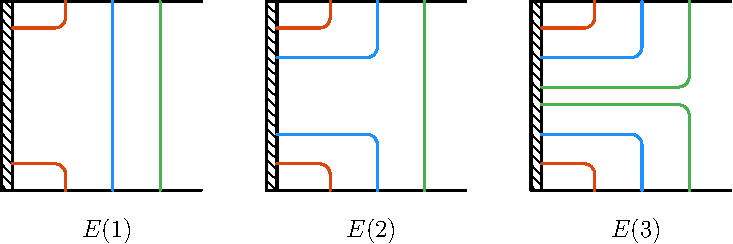
\includegraphics[width=0.72\textwidth]{figures/fig-fusscatalan-generators.pdf}
    \caption{The first three boundary generators of the Fuss--Catalan algebra,
    written $E(s)$ for $E_2^{(s)}$: each attaches the innermost one, two, or
    three coloured strands of the boundary bundle to the wall (hatched). These
    are the objects whose spectral-parameter-dependent coefficients are
    classified here. Theorem~\ref{thm:main} states that $E(3)$, and every
    deeper generator at higher rank, carries the coefficient zero.}
    \label{fig:boundary-generators}
\end{figure*}

Three scalars weight the closed loops that stacking creates: the bulk weight
$t$, and the weights $e$ and $o$ carried respectively by even-to-odd and
odd-to-even boundary loops, written $\tau,\tau_e,\tau_o$ in
Ref.~\cite{shigechi2025fuss}. We parametrize them by two algebraically
independent variables $q$ and $q_2$,
\begin{equation}
  t=-(q+q^{-1}),\qquad e=-(q_2+q_2^{-1}),\qquad o=\frac{q}{q_2}+\frac{q_2}{q},
  \label{eq:weights}
\end{equation}
which is the general solution of the single constraint the three weights of a
Fuss--Catalan algebra must satisfy,
\begin{equation}
  t^2+e^2+o^2-teo-4=0 .
  \label{eq:fc-constraint}
\end{equation}
Two of the three loop weights may thus be chosen freely and the third is then
determined up to the exchange encoded in~\eqref{eq:weights}. All coefficients
below live in the field
\begin{equation}
  \Fld=\mathbb{C}(q,q_2),
  \label{eq:field}
\end{equation}
the smallest field containing the loop weights, localized at the denominators
displayed as they arise. Four combinations of the weights recur often enough to
be abbreviated once and for all,
\begin{equation}
  T=t^2-1,\qquad L=t^2-2,\qquad A=te-o,\qquad B=to-e ,
  \label{eq:abbrev}
\end{equation}
each of which is a polynomial in the loop weights and none of which vanishes
identically. Products of two boundary generators at the same site reduce to a
single one,
\begin{equation}
  E_2^{(s)}E_2^{(u)}=e^{\min(s,u)}E_2^{(\max(s,u))},
  \label{eq:boundary-products}
\end{equation}
because stacking a shallower attachment onto a deeper one closes
$\min(s,u)$ loops and leaves the deeper attachment behind; the same rule with
$e$ replaced by $t$ holds at the bulk site.

One consequence of~\eqref{eq:boundary-products} is used repeatedly. For a
boundary operator $1+\sum_s k_s(w)E_2^{(s)}$ define the cumulative quantities
\begin{equation}
  \lambda_j(w)=1+\sum_{s=1}^{j}e^{s}k_s(w),\qquad \lambda_0=1 ,
  \label{eq:cumulative}
\end{equation}
which are the eigenvalues the operator would have on a state where the
innermost $j$ strands are already attached to the wall: only the generators up
to depth $j$ act, and each contributes its coefficient times the loop weight it
collects.

\subsection{The bulk operator}

A row-to-row transfer matrix collects the local Boltzmann weights along one row
of the lattice, and the model is integrable when transfer matrices at different
values of the spectral parameter commute, since the family then generates
infinitely many conserved quantities. The standard sufficient condition is a
one-parameter family of local operators $R_i(x)$ acting on the neighbouring
sites $i,i+1$ and satisfying the Yang--Baxter equation, written here in the
multiplicative convention of Refs.~\cite{di1998new,shigechi2025fuss},
\begin{equation}
  R_i(x)\,R_{i+1}(xy)\,R_i(y)=R_{i+1}(y)\,R_i(xy)\,R_{i+1}(x).
  \label{eq:ybe}
\end{equation}
Both sides move three world lines past one another, and the equation says that
the order in which the crossings are performed does not matter.

The bulk structure used here is Di Francesco's fundamental
branch~\cite{di1998new}. Translating his generators into the normalization of
Ref.~\cite{shigechi2025fuss} cancels an auxiliary square root and gives, for
every $r\ge2$,
\begin{equation}
  R_i^{(r)}(x)=1+\sum_{s=1}^{r-1}
  \frac{x^{s-1}(x-1)}{t^s}E_i^{(s)}
  +\frac{x^{r-1}(x-1)}{t^{r-2}(T-x)}E_i^{(r)} .
  \label{eq:rmatrix}
\end{equation}
Every colour below the top contributes a coefficient that is a polynomial in
the spectral parameter, and only the top colour carries a pole, at $x=T$; this
single pole is what makes each new rank a genuinely new problem rather than a
copy of the previous one. The operator satisfies $R_i^{(r)}(1)=1$ and
$R_i^{(r)}(x)R_i^{(r)}(x^{-1})=1$, so it reduces to the identity at the
symmetric point and undoes itself under inversion of the spectral parameter.
Di Francesco's excited branches, which first exist at $r=4$, have different
coefficients and define different boundary problems; they are outside the scope
of this paper.

\subsection{The reflection equation and the problem}

A boundary operator acts at the wall and depends on its own spectral parameter.
It preserves integrability when it satisfies the right reflection equation,
Eq.~(9.2) of Ref.~\cite{shigechi2025fuss},
\begin{equation}
  \begin{split}
  K_2^{(r)}(w)\,&R_1^{(r)}\!\left((wz)^{-1}\right)
  K_2^{(r)}(z)\,R_1^{(r)}(w/z)\\
  &=R_1^{(r)}(w/z)\,K_2^{(r)}(z)\,
  R_1^{(r)}\!\left((wz)^{-1}\right)K_2^{(r)}(w).
  \end{split}
  \label{eq:re}
\end{equation}
Two world lines carrying spectral parameters $w$ and $z$ approach the wall,
cross each other twice and bounce off the wall once each; the equation says
that the two possible orders of those four events produce the same operator.
By Sklyanin's construction~\cite{sklyanin1988boundary}, a solution
of~\eqref{eq:re} together with~\eqref{eq:ybe} guarantees an infinite commuting
family of double-row transfer matrices on a strip, one row of bulk operators
carrying the system towards the wall and a second carrying it back.

The object to be classified is
\begin{equation}
  K_2^{(r)}(w)=1+\sum_{s=1}^{r}k_s(w)E_2^{(s)} ,
  \label{eq:ansatz}
\end{equation}
the general element of the boundary subalgebra with identity coefficient one,
its $r$ coefficients being meromorphic functions of $w$. Fixing the identity
coefficient fixes the overall scale, which the reflection equation leaves free.
We require, besides~\eqref{eq:re}, that
\begin{equation}
  K_2^{(r)}(1)=1,\qquad
  K_2^{(r)}(w)K_2^{(r)}(w^{-1})=1 ,
  \label{eq:conditions}
\end{equation}
so that the boundary is transparent at the symmetric point and undoes itself
under inversion, matching the two properties the bulk operator already has.
Classifying means more than exhibiting solutions: both sides of~\eqref{eq:re}
must be reduced to a basis of the algebra and the resulting equations
eliminated, so that the branches found are shown to exhaust the ansatz.

\section{The classification}
\label{sec:theorem}

\begin{theorem}
\label{thm:main}
Let $t,e,o$ be as in~\eqref{eq:weights} with $q,q_2$ algebraically independent,
let $\Fld=\mathbb{C}(q,q_2)$, fix an integer $r\ge3$, and take the fundamental
bulk operator~\eqref{eq:rmatrix}. Then every $K_2^{(r)}$ of the
form~\eqref{eq:ansatz} with meromorphic coefficients satisfying the reflection
equation~\eqref{eq:re} and the conditions~\eqref{eq:conditions}, over $\Fld$
localized away from the zero loci listed in Sec.~\ref{sec:discussion}, has
\begin{equation}
  k_s\equiv0\qquad\text{for every }s\ge3 ,
  \label{eq:no-deep}
\end{equation}
so no boundary generator deeper than the second occurs, and is exactly one of
the following.
\begin{enumerate}
\item[\textup{(a)}] \emph{The identity.} $k_s\equiv0$ for every $s$, that is
$K_2^{(r)}(w)=1$.
\item[\textup{(b)}] \emph{A one-constant family.} For a constant $C$
independent of $w$,
\begin{equation}
  k_1(w)=\frac{L\,(w^2-1)}{\Xi_C(w)},\qquad
  k_s(w)=0\quad(2\le s\le r),
  \label{eq:free-family}
\end{equation}
where $\Xi_C(w)=B+Cw-(eT-to)w^2$. This satisfies $K_2^{(r)}(1)=1$ if and only
if
\begin{equation}
  C\ne t^2e-2to .
  \label{eq:free-normalization}
\end{equation}
\end{enumerate}
Set
\begin{equation}
  \begin{gathered}
  \Disc=\frac{eoT\,A}{B},\qquad S=\frac{aB}{T},\\
  Q_a(w)=S-e\left\{a w^2+(te-2o)\,w\right\}
  \end{gathered}
  \label{eq:disc}
\end{equation}
for either root $a$ of $a^2=\Disc$. Over the extension $\Fld(a)$ the families
\textup{(a)} and \textup{(b)} persist with their constants in the larger field,
and exactly two further branches appear, one for each sign of $a$:
\begin{enumerate}
\item[\textup{(c,d)}] \emph{A conjugate pair.}
\begin{equation}
  k_1(w)=\frac{(a w-o)(w^2-1)}{w\,Q_a(w)},\qquad
  k_2(w)=\frac{t\,(w^2-1)}{w\,Q_a(w)},
  \label{eq:algebraic-branch}
\end{equation}
with $k_s\equiv0$ for $3\le s\le r$. Each satisfies $K_2^{(r)}(1)=1$ if and
only if $Q_a(1)=S-e(a+te-2o)\ne0$, which holds for both signs on the generic
locus.
\end{enumerate}
The extension is genuine: $\Disc$ is not a square in $\Fld$. The minimal field
over which each branch is defined is $\Fld$ for \textup{(a)}, $\Fld(C)$ for a
branch \textup{(b)} with $C\neq 0$, and $\Fld(\sqrt{\Disc})$ for each of
\textup{(c,d)}.
\end{theorem}

Figure~\ref{fig:k-classification} summarizes the statement. Three features of
it are worth separating. The list does not depend on $r$: the same four
branches occur at three colours and at three hundred, and nothing new is
gained by making the bundle deeper. The two conditions
in~\eqref{eq:conditions} play different roles: $K_2^{(r)}(1)=1$ selects which
members of each family survive, while the inversion identity turns out to hold
automatically on every branch the reflection equation produces, as
Sec.~\ref{sec:unitarity} shows. And a member excluded by the normalization is
not thereby singular: it can remain meromorphic and regular at $w=1$ while
taking a value there other than the identity.

\begin{figure*}[htbp]
    \centering
    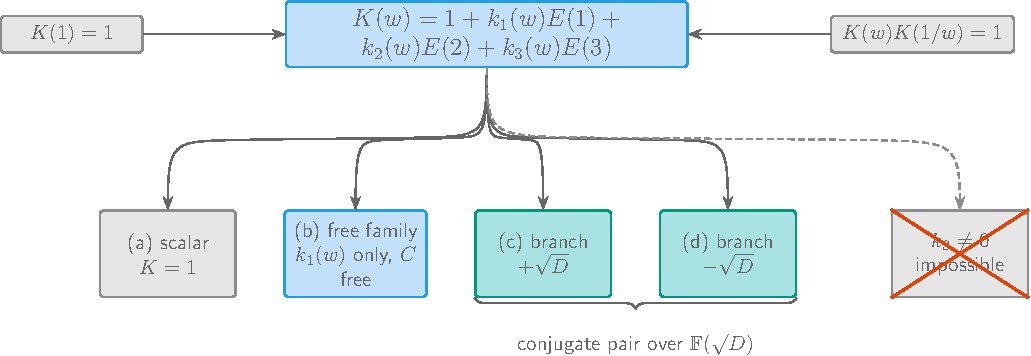
\includegraphics[width=\textwidth]{figures/fig-kmatrix-classification.pdf}
    \caption{The classification of Theorem~\ref{thm:main}, with $E(s)$ written
    for $E_2^{(s)}$ and $D$ for $\Disc$. Whatever the rank $r\ge3$, the
    identity-normalized solutions of the reflection equation are the identity,
    a family carrying one free constant $C$ and supported on $E(1)$ alone, and
    a conjugate pair supported on $E(1)$ and $E(2)$ that exists only over the
    quadratic extension $\Fld(\sqrt{\Disc})$. The branch reaching the third
    generator, and every deeper one, is empty.}
    \label{fig:k-classification}
\end{figure*}

\begin{example}
\label{ex:concrete}
At $(q,q_2)=(2,3)$ the loop weights~\eqref{eq:weights} are
$(t,e,o)=(-5/2,\,-10/3,\,13/6)$. Taking $C=7$ in~\eqref{eq:free-family} gives
\begin{equation*}
  k_1(w)=\frac{51\,(w^2-1)}{145w^2+84w-25},\qquad
  k_s=0\quad(2\le s\le r),
\end{equation*}
whose denominator does not vanish at $w=1$, so this member is normalized and
regular. The proofs below are exact rather than numerical; the example is here
only to make the statement concrete.
\end{example}

\section{The rank-three base case}
\label{sec:base}

\subsection{A complete diagram basis}

Reduction inside the algebra is governed, colour by colour, by three rules. For
a single colour, writing $e_1$ for the bulk generator and $b$ for the boundary
generator,
\begin{equation}
  e_1^2=t\,e_1,\qquad b^2=e\,b,\qquad e_1be_1=o\,e_1 ,
  \label{eq:single-colour}
\end{equation}
each of which removes one letter in exchange for a loop weight: the first
closes a bulk loop, the second a boundary loop, and the third the boundary loop
that a strand makes by leaving the wall and returning.

\begin{lemma}
\label{lem:basis}
The rewriting system~\eqref{eq:single-colour} leaves exactly six one-colour
normal words,
\begin{equation}
  1,\quad e_1,\quad b,\quad e_1b,\quad be_1,\quad be_1b ,
  \label{eq:normal-words}
\end{equation}
and the admissible three-colour triples of these number exactly $36$, which is
the dimension of $\BFCthree$. Hence the $36$ normal triples are a basis, and
two elements of $\BFCthree$ are equal if and only if all $36$ of their
coefficients agree.
\end{lemma}

\begin{proof}
A word in $e_1$ and $b$ is normal when it contains no factor $e_1e_1$, $bb$, or
$e_1be_1$; since the letters alternate in a normal word and the word cannot
contain two consecutive equal letters, a normal word is determined by its
length and its first letter, and the rules forbid length beyond three. That
leaves the six words in~\eqref{eq:normal-words}. Nesting of the strand bundles
restricts which triples occur: a letter of colour $s$ may be followed by a
letter of colour $s+1$ only when the shorter word ends on the boundary, and
preceded by one only when the longer word begins there. Imposing this condition
on the $6^3=216$ unrestricted triples leaves $36$, as counted in
Appendix~\ref{app:normal-forms}. Since every word reduces to one of the $36$
and their number equals the dimension the algebra has by Proposition~7.3 of
Ref.~\cite{shigechi2025fuss}, no relation among them survives, and they form a
basis.
\end{proof}

The point of Lemma~\ref{lem:basis} is that the count is exact rather than an
upper bound. Equating $36$ coefficients is therefore equality in the abstract
algebra and not merely in some representation of it, a distinction that decides
whether a classification is complete: a proof carried out inside a
representation would leave open whether further solutions live in its kernel.

\subsection{The coefficient inventory}

\begin{lemma}
\label{lem:inventory}
Expanded in the basis of Lemma~\ref{lem:basis}, the difference of the two sides
of the reflection equation~\eqref{eq:re} at $r=3$ has exactly $20$ coefficients
that are not identically zero. They occur in ten pairs related by exchanging
$w$ and $z$ and reversing the overall sign, so the reflection equation is
equivalent to the vanishing of ten functional equations in $k_1,k_2,k_3$.
\end{lemma}

\begin{proof}
The proof is an exhaustive computation, carried out symbolically over $\Fld$
and over the field of rational functions in $w$ and $z$.

Each case is one of the $36$ normal triples of Lemma~\ref{lem:basis} --- an
explicit word such as $\mathtt{beb}\,|\,\mathtt{eb}\,|\,\mathtt{b}$, one
one-colour normal word for each of the three colours. The reflection difference
is a single element of $\BFCthree$ whose coefficients are rational functions of
$t,e,o,w,z$ and of the six unknowns $k_s(w),k_s(z)$; expanding it means
applying the rules~\eqref{eq:single-colour} and~\eqref{eq:boundary-products},
together with the concatenation rule for mixed colours, until every product is
a normal triple.

The test applied to a case is whether its coefficient reduces to the zero
rational function. This is decisive because the rewriting system is confluent
--- the three rules shorten every word and overlap only in ways that reduce to
the same normal word --- so the reduced coefficient of a normal triple is
unique, and by Lemma~\ref{lem:basis} the reflection difference vanishes in the
algebra precisely when all $36$ reduce to zero. The cases are exhaustive
because Lemma~\ref{lem:basis} enumerates the basis in full: there are $36$
normal triples and no others, and every product occurring in~\eqref{eq:re}
reduces to a combination of them.

Sixteen coefficients reduce to zero identically. The remaining $20$ do not, and
inspection of them shows that each is carried to the negative of another by the
substitution $w\leftrightarrow z$, which pairs them into ten classes. Since a
function and its reversal vanish together, ten independent equations remain.
\end{proof}

Everything that follows at rank three is elimination on those ten equations.
They split into three mutually exclusive and jointly exhaustive cases according
to which of the coefficients vanish identically: $k_3\not\equiv0$; $k_3\equiv0$
with $k_2\not\equiv0$; and $k_2\equiv k_3\equiv0$. We take them in turn.

\subsection{No solution reaches the third colour}
\label{sec:k3}

\begin{proposition}
\label{prop:k3}
At $r=3$ and on the generic locus, no solution of~\eqref{eq:re} has
$k_3\not\equiv0$.
\end{proposition}

\begin{proof}
Write $h=k_3$ and divide by it, which is legitimate because the branch
$h\equiv0$ has already been separated off and because an identity between
meromorphic functions valid off the isolated zeros of $h$ extends across them.
The two coefficients of Lemma~\ref{lem:inventory} carrying the shortest normal
words give
\begin{equation}
  k_2(u)=\frac{\gamma u-o}{t}\,h(u),\qquad
  k_1(u)=\left(\delta u^2-\frac{o\gamma}{t^2}\,u\right)h(u)
  \label{eq:k3-reduction}
\end{equation}
for constants $\gamma,\delta$ that do not depend on the spectral parameter:
each of those two coefficients states that a function of $u$ takes the same
value at $w$ and at $z$, which forces it to be constant. So the two lower
coefficients are determined by the top one up to two numbers.

Introduce
\begin{equation}
  \begin{gathered}
  g(u)=\frac{u^2-1}{u\,h(u)},\\
  \Psi(u)=\delta t^2(u^3-u)+\gamma\,A\,u^2+(t^2e^2-2teo)\,u ,
  \end{gathered}
  \label{eq:k3-g}
\end{equation}
the first being the natural variable in which the remaining equations
linearize, and the second a cubic polynomial in the spectral parameter built
from the two constants. A fifth coefficient becomes the separated statement
$g(w)-g(z)=-(e/t^2)\{\Psi(w)-\Psi(z)\}$, whose complete meromorphic solution is
\begin{equation}
  g(u)=\ell-\frac{e}{t^2}\Psi(u)
  \label{eq:k3-gsol}
\end{equation}
for a single constant $\ell$; a difference depending only on $u$ on each side
fixes the function up to an additive constant. Substituting~\eqref{eq:k3-gsol}
into the successive coefficients then forces
\begin{equation}
  \ell=0,\qquad \gamma^2=te\,A,\qquad \delta t^2A=e^2T(te-2o),
  \label{eq:k3-constraints}
\end{equation}
so all three constants are pinned, the last two only up to the sign of
$\gamma$.

These necessary conditions are inconsistent with a further coefficient. After
imposing~\eqref{eq:k3-constraints} its residual is a nonzero multiple of
\begin{equation}
  H_{\mathrm{obs}}=\frac{H_1H_2}{q^6q_2^4} ,
  \label{eq:hobs}
\end{equation}
where $H_1$ and $H_2$ are the polynomials in $\mathbb{Z}[q,q_2]$ recorded in
Appendix~\ref{app:obstruction}, so the branch survives only where
$H_{\mathrm{obs}}$ vanishes. Neither factor is the zero polynomial, which a
single specialization certifies:
\begin{equation}
  H_{\mathrm{obs}}(2,3)=\frac{13438225}{5184}\ne0 .
  \label{eq:hobs-value}
\end{equation}
A polynomial with one nonzero value is not the zero polynomial, and since $q$
and $q_2$ are algebraically independent, $H_{\mathrm{obs}}\neq0$ in $\Fld$.
The branch is therefore empty.
\end{proof}

Proposition~\ref{prop:k3} is the step with no counterpart at one or two
colours, where there is no third generator to use. It is what forbids a
boundary operator from reaching all three strands of the bundle, and the reason
the classification below is so much more rigid than its one-colour analogue.

\subsection{The conjugate pair}

\begin{proposition}
\label{prop:k2}
At $r=3$, on the generic locus and with $k_3\equiv0$, every solution with
$k_2\not\equiv0$ is one of the two branches~\eqref{eq:algebraic-branch}.
\end{proposition}

\begin{proof}
One coefficient of Lemma~\ref{lem:inventory} forces
\begin{equation}
  k_1(u)=\frac{au-o}{t}\,k_2(u)
  \label{eq:k2-ratio}
\end{equation}
for a constant $a$, by the same argument that
gave~\eqref{eq:k3-reduction}: the shallower coefficient is a fixed
spectral-parameter-dependent multiple of the deeper one. Writing
$g_2(u)=(u^2-1)/\{u\,k_2(u)\}$, the next functional equation separates and has
the complete meromorphic solution
\begin{equation}
  g_2(u)=\ell_2-\frac{e}{t}\left\{au^2+(te-2o)u\right\},
  \label{eq:k2-g}
\end{equation}
a quadratic in the spectral parameter with one free additive constant. The
remaining coefficients are together equivalent to the two conditions
\begin{equation}
  \ell_2=\frac{aB}{tT},\qquad a^2B=eoT\,A ,
  \label{eq:k2-constraints}
\end{equation}
which fix the additive constant to $S/t$ and force $a^2=\Disc$ with $\Disc$ as
in~\eqref{eq:disc}. Substituting back through~\eqref{eq:k2-ratio}
and~\eqref{eq:k2-g} gives exactly~\eqref{eq:algebraic-branch}, and with those
coefficients all $20$ coefficients of Lemma~\ref{lem:inventory} vanish
identically, so these are solutions and not merely candidates. The two roots
$a=\pm\sqrt{\Disc}$ give the two conjugate branches.
\end{proof}

\subsection{The one-constant family and the identity}

\begin{proposition}
\label{prop:k1}
At $r=3$, on the generic locus and with $k_2\equiv k_3\equiv0$, the solutions
are exactly the family~\eqref{eq:free-family} and the identity.
\end{proposition}

\begin{proof}
Exactly one of the ten equations survives, namely
\begin{equation}
  \begin{split}
  -Lw&(z^2-1)k_1(w)+Lz(w^2-1)k_1(z)\\
  &+(w-z)\left\{(eT-to)wz+B\right\}k_1(w)k_1(z)=0 .
  \end{split}
  \label{eq:k1-eq}
\end{equation}
It is a single quadratic functional equation relating the one remaining
coefficient at two spectral parameters. Setting $g_1(u)=(u^2-1)/\{u\,k_1(u)\}$
turns it into the separated form
\begin{equation}
  g_1(w)-g_1(z)=-\frac{w-z}{L}\left(eT-to+\frac{B}{wz}\right),
  \label{eq:k1-separated}
\end{equation}
in which each side depends on $w$ and $z$ only through a difference of
functions of one variable. Its complete meromorphic solution carries a single
integration constant $C$ and yields~\eqref{eq:free-family}. If instead
$k_1\equiv0$ the operator is the identity. The three branch splits are mutually
exclusive and jointly exhaustive, and meromorphic continuation covers the
isolated zeros used in each division, so together with
Propositions~\ref{prop:k3} and~\ref{prop:k2} this classifies rank three.
\end{proof}

\section{Lowering the rank by one colour}
\label{sec:peeling}

Rank three is now settled, and the task is to reach every higher rank without
expanding diagram bases whose dimension grows with $r$. The mechanism is a map
that adds colours to the outside of the bundle, and it is exact rather than
asymptotic.

\begin{lemma}
\label{lem:peeling}
Let $r=m+p$ with $m\ge2$ and $p\ge1$. Writing $E_i^{(j)}$ for the generators of
$\BFCm$ on the left and of $\BFC$ on the right, the assignment
\begin{equation}
  \Phi_p(E_1^{(j)})=t^{-p}E_1^{(p+j)},\qquad
  \Phi_p(E_2^{(j)})=E_2^{(j)}
  \label{eq:phi}
\end{equation}
extends to an injective algebra homomorphism $\BFCm\to\BFC$. With
\begin{equation}
  P_p(x)=1+\sum_{s=1}^{p}\frac{x^{s-1}(x-1)}{t^s}E_1^{(s)}
  \label{eq:prefix}
\end{equation}
the fundamental bulk operators at the two ranks are related by
\begin{equation}
  R^{(r)}(x)=P_p(x)\,\Phi_p\!\left(R^{(m)}(x)\right),
  \label{eq:bulk-factorization}
\end{equation}
and $P_p(x)P_p(x^{-1})=1$. Consequently, for a boundary operator supported on
the first $m$ generators, the difference $\Delta_n$ of the two sides of the
rank-$n$ reflection equation obeys
\begin{equation}
  \Delta_r(w,z)=P_p(v)P_p(u)\,\Phi_p\!\left(\Delta_m(w,z)\right)
  \label{eq:reflection-factorization}
\end{equation}
with $u=w/z$ and $v=(wz)^{-1}$, so the rank-$r$ reflection equation holds if
and only if the rank-$m$ one does, and the same for
both conditions in~\eqref{eq:conditions}.
\end{lemma}

\begin{proof}
Write a normal word of $\BFCm$ in the tensor-word notation of
Lemma~\ref{lem:basis}. A word containing no bulk letter maps under $\Phi_p$ to
$W\otimes1^{\otimes p}$, while a word containing one maps to
$t^{-p}W\otimes\mathtt{e}^{\otimes p}$; distinct normal words stay distinct, so
$\Phi_p$ is injective. For multiplicativity, if both factors contain a bulk
letter then the tail contributes $(\mathtt{e}^{\otimes p})^2=t^{p}\,
\mathtt{e}^{\otimes p}$, which cancels one of the two factors $t^{-p}$; the
cases with one or no bulk-containing factor are immediate. So $\Phi_p$ embeds
the smaller algebra as the sub-bundle of the $p$ innermost colours.

For~\eqref{eq:bulk-factorization}, the same-site product rule and the identity
$1+\sum_{s=1}^{p}t^sx^{s-1}(x-1)/t^s=x^{p}$ give, on the right-hand side, the
coefficient $t^{-p}x^{p}\,x^{j-1}(x-1)/t^{j}$ for $E_1^{(p+j)}$ with $j<m$ and
the top coefficient of~\eqref{eq:rmatrix} for $j=m$; together with the levels
already in~\eqref{eq:prefix} these are every coefficient of the left-hand side.
Thus the rank-$r$ bulk operator splits into a part acting only on the $p$ outer
colours and the image of the rank-$m$ operator.

The cumulative eigenvalues of $P_p(x)$, computed
from~\eqref{eq:cumulative} with $e$ replaced by $t$, are $x^j$ for $j\le p$ and
$x^{p}$ beyond, all of which invert under $x\mapsto x^{-1}$; hence
$P_p(x)^{-1}=P_p(x^{-1})$. Moreover $P_p$ commutes with the embedded bulk
operator and with every $E_2^{(j)}$ for $j\le m$, since each relevant pair of
depths satisfies $s+j\le p+m=r$ and the two attachments then act on disjoint
strands. Moving the commuting prefixes to the left in~\eqref{eq:re}
gives~\eqref{eq:reflection-factorization}. Since $P_p(v)P_p(u)$ is invertible
and $\Phi_p$ injective, $\Delta_r$ vanishes exactly when $\Delta_m$ does, and
because $\Phi_p$ fixes the boundary generators it carries $K^{(m)}(1)=1$ and
the inversion identity to their rank-$r$ counterparts and back.
\end{proof}

The content of Lemma~\ref{lem:peeling} is that the outer colours of the bundle
are inert as long as the boundary does not reach them: a rank-$r$ problem whose
boundary stops at depth $m$ is not merely similar to the rank-$m$ problem, it
is that problem. What remains is to show that the boundary never does reach the
outer colours.

\section{No boundary reaches the top colour}
\label{sec:primitive}

\subsection{The four-colour obstruction}

Two bulk operators must be treated together. Besides the fundamental
$R^{(4)}$ of~\eqref{eq:rmatrix}, introduce the truncated four-colour operator
\begin{equation}
  \widetilde R^{(4)}(x)
  =1+\sum_{s=1}^{4}\frac{x^{s-1}(x-1)}{t^s}E_1^{(s)} ,
  \label{eq:truncated-r4}
\end{equation}
which differs from $R^{(4)}$ only in the top coefficient, having no pole. The
truncated operator is not itself a bulk solution of interest; it is what the
projection of the next subsection produces from every rank above four, so both
must be excluded.

\begin{table*}[htbp]
\caption{The four coefficients of the four-colour reflection difference used in
the proof of Proposition~\ref{prop:r4}. Each row names the normal word whose
coefficient is taken, the monomial in the spectral parameters whose coefficient
inside it is extracted, and the factor that must then vanish. The factors are
identical for the fundamental operator $R^{(4)}$ and for the truncated operator
$\widetilde R^{(4)}$.}
\label{tab:r4}
\begin{ruledtabular}
\begin{tabular}{lll}
normal word & monomial & necessary factor\\
\hline
$\mathtt{b|b|be|be}$ & $wz^2$ & $\ell_4 t^2$\\
$\mathtt{b|b|be|e}$ & $w^3z^5$ & $e^2(\gamma_4^2o-t^3e-te^3+4te)$\\
$\mathtt{b|be|be|be}$ & $w^2z^3$ & $t^2e(\delta_4A-te^3+2e^2o)$\\
$\mathtt{b|be|e|e}$ & $w^7z^6$ & $t^2eo(\gamma_4e-\delta_4t)(\gamma_4e+\delta_4t)$\\
\end{tabular}
\end{ruledtabular}
\end{table*}

\begin{proposition}
\label{prop:r4}
On the generic locus, neither the four-colour reflection problem for $R^{(4)}$
nor the one for $\widetilde R^{(4)}$ has an identity-normalized meromorphic
solution with $k_4\not\equiv0$.
\end{proposition}

\begin{proof}
Set $h=k_4$ and $f_j=k_j/h$, dividing where the divisor is nonzero and
extending meromorphically as before. For both bulk operators, the three
coefficients of the reflection difference carrying the normal words
$\mathtt{beb|beb|beb|eb}$, $\mathtt{beb|beb|eb|eb}$ and
$\mathtt{beb|eb|eb|eb}$ give successively
\begin{align}
 tzf_3(w)-twf_3(z)+o(z-w)&=0,\nonumber\\
 t^2\{z^2f_2(w)-w^2f_2(z)\}+o\gamma_4wz(z-w)&=0,\nonumber\\
 t^3\{z^3f_1(w)-w^3f_1(z)\}+o\delta_4t^2w^2z^2(z-w)&=0 .
 \label{eq:r4-chain}
\end{align}
Each equation says that one function of a single variable takes equal values at
$w$ and at $z$, hence is constant, so with constants
$\alpha_4,\gamma_4,\delta_4$ independent of the spectral parameter,
\begin{equation}
 \begin{gathered}
 f_3(x)=\frac{\gamma_4x-o}{t},\qquad
 f_2(x)=\delta_4x^2-\frac{o\gamma_4}{t^2}x,\\
 f_1(x)=\alpha_4x^3-\frac{o\delta_4}{t}x^2 .
 \end{gathered}
 \label{eq:r4-ratios}
\end{equation}
Each shallower coefficient is thus a fixed polynomial multiple of the top one,
with one new constant appearing at each depth.

With $g_4(x)=(x^2-1)/\{x\,h(x)\}$ the coefficient of $\mathtt{b|b|b|be}$
separates and gives
\begin{equation}
 g_4(x)=\ell_4-\frac{e}{t^2}\Psi_4(x),
 \label{eq:r4-master}
\end{equation}
where
\begin{equation}
\begin{split}
 \Psi_4(x)={}&\alpha_4t^2(x^4-x^2)+\gamma_4(te^2-eo)x^2\\
 &+\delta_4(t^2e-to)(x^3-x)+(t^2e^3-2te^2o)x
\end{split}
 \label{eq:psi4}
\end{equation}
is a quartic polynomial in the spectral parameter assembled from the three
constants. So the top coefficient is itself determined up to one further
constant $\ell_4$, and the entire boundary operator now depends on four
numbers.

Four more coefficients suffice to contradict that. Substituting
\eqref{eq:r4-ratios} and~\eqref{eq:r4-master}, clearing the bulk denominators
displayed in~\eqref{eq:rmatrix} and~\eqref{eq:truncated-r4} and reducing
modulo the constraint~\eqref{eq:fc-constraint}, the coefficients listed in
Table~\ref{tab:r4} carry the factors printed there, identically for the two
bulk operators. On the generic locus, where $t$, $e$, $o$ and $A$ do not
vanish, these force
\begin{equation}
 \ell_4=0,\quad \gamma_4^2=teA,\quad
 \delta_4A=e^2(te-2o),\quad \gamma_4^2e^2=\delta_4^2t^2 ,
 \label{eq:r4-constraints}
\end{equation}
where the second uses $t^2+e^2-4=oA$, a rearrangement
of~\eqref{eq:fc-constraint}. The three unknown constants are thereby
overdetermined: eliminating $\gamma_4$ and $\delta_4$ from the last three
conditions leaves a relation among the loop weights alone,
\begin{equation}
 H_4=A^3-te(te-2o)^2=0 .
 \label{eq:h4}
\end{equation}
That relation is false. In the parametrization~\eqref{eq:weights},
\begin{equation}
\begin{split}
 H_4=\frac{1}{q^3q_2^3}\,(q^2+q_2^2)\,\bigl(&q^4q_2^4+q^4q_2^2-q^4\\
 &+q^2q_2^4+q^2-q_2^4+q_2^2+1\bigr),
\end{split}
 \label{eq:h4-factor}
\end{equation}
and $H_4(2,3)=21853/216\ne0$, so $H_4$ is not the zero element of $\Fld$.
Hence no such solution exists for either bulk operator.
\end{proof}

The elimination in Proposition~\ref{prop:r4} rests on a finite exhaustive
expansion of the same kind as Lemma~\ref{lem:inventory}, one rank higher. Each
case is a four-colour normal word; the test is whether its coefficient reduces
to zero; the reduction is decisive because the four-colour normal words are
again a basis, obtained from the same rewriting system; and the cases are
exhaustive because every product in the reflection equation reduces to a
combination of them. The full expansion has $40$ coefficients that are not
identically zero, falling into $20$ reversal pairs, for each of the two bulk
operators; the four rows of Table~\ref{tab:r4} are the ones the argument uses,
and the remaining coefficients are consistent with, and add nothing to,
\eqref{eq:r4-constraints}.

\subsection{Transporting the obstruction to every rank}

\begin{lemma}
\label{lem:projection}
Let $r=p+4$ with $p\ge1$. Projecting the reflection difference onto normal
words whose $p$ outermost colours are exactly $\mathtt{b}$ and deleting that
prefix gives
\begin{equation}
 \Pi_p(\Delta_r)=
 \frac{\lambda_p(w)\lambda_p(z)}{e^{p}}\,
 \Delta_{\widetilde R^{(4)}}\!\left(\widehat K(w),\widehat K(z)\right),
 \label{eq:prefix-projection}
\end{equation}
where $\lambda_p$ is the cumulative quantity~\eqref{eq:cumulative}, the right
side is the four-colour reflection difference for the truncated operator, and
\begin{equation}
 \widehat K(x)=1+\sum_{j=1}^{4}\widehat k_j(x)E_2^{(j)},\qquad
 \widehat k_j(x)=\frac{e^{p}k_{p+j}(x)}{\lambda_p(x)} .
 \label{eq:effective-k}
\end{equation}
\end{lemma}

\begin{proof}
No word containing the bulk letter $\mathtt{e}$ can reduce to a word of
$\mathtt{b}$ alone: each rule $\mathtt{ee}\mapsto t\,\mathtt{e}$,
$\mathtt{bb}\mapsto e\,\mathtt{b}$ and $\mathtt{ebe}\mapsto o\,\mathtt{e}$
leaves a bulk letter behind whenever one is present. Every bulk level above the
fourth therefore drops out of this sector, and the first four bulk levels
of~\eqref{eq:rmatrix} become exactly~\eqref{eq:truncated-r4} on the remaining
colours: the projection removes the outer colours and, with them, the pole that
distinguished the fundamental operator from the truncated one.

On the boundary side, a term of depth at most $p$ multiplying the full prefix
$\mathtt{b}^{\otimes p}$ contributes precisely the scalar $\lambda_p$ by the
same-site rule~\eqref{eq:boundary-products}; two full-prefix terms contribute
the factor $e^{p}$; and the contribution in which both boundary factors stay
below the prefix is proportional to the commutator of the two bulk operators,
which vanishes. Expanding the remaining cases
gives~\eqref{eq:prefix-projection}. The identity normalization forces
$\lambda_p(1)=1$, so $\lambda_p$ is not the zero function and the division
in~\eqref{eq:effective-k} is legitimate as an identity of meromorphic
functions.
\end{proof}

\begin{proposition}
\label{prop:no-top}
For every $r\ge4$, every identity-normalized meromorphic solution of the
rank-$r$ reflection equation on the generic locus has $k_r\equiv0$.
\end{proposition}

\begin{proof}
At $r=4$ this is Proposition~\ref{prop:r4}. For $r\ge5$, suppose
$k_r\not\equiv0$. Then $\widehat k_4\not\equiv0$
in~\eqref{eq:effective-k}, and Lemma~\ref{lem:projection} turns the solution
into an identity-normalized solution of the four-colour problem for
$\widetilde R^{(4)}$ with nonvanishing top coefficient, which
Proposition~\ref{prop:r4} forbids.
\end{proof}

\section{Proof of the classification}
\label{sec:induction}

\begin{proof}[Proof of Theorem~\ref{thm:main}]
Fix $r\ge3$ and a solution. If $r\ge4$, Proposition~\ref{prop:no-top} gives
$k_r\equiv0$, and Lemma~\ref{lem:peeling} with $m=r-1$ and $p=1$ identifies the
remaining boundary operator with a solution of the rank-$(r-1)$ problem,
carrying both conditions~\eqref{eq:conditions} across. Iterating lowers the
rank one colour at a time until $r=3$ is reached, where
Propositions~\ref{prop:k3}, \ref{prop:k2} and~\ref{prop:k1} leave exactly the
branches \textup{(a)}--\textup{(d)}, all of which have $k_3\equiv0$. Tracing
the iteration back gives~\eqref{eq:no-deep}.

Conversely, each rank-three branch lifts. Applying
Lemma~\ref{lem:peeling} in the other direction with $m=3$ and $p=r-3$ shows
that the same coefficients $k_1,k_2$, with every deeper coefficient zero, solve
the rank-$r$ reflection equation, since $\Delta_r$ is the image of $\Delta_3$
under an injective map composed with an invertible factor. So the four branches
occur at every rank and nothing else does. The statements about normalization,
the inversion identity and the minimal fields are proved in
Sec.~\ref{sec:unitarity}.
\end{proof}

\section{Inversion, normalization, and minimal fields}
\label{sec:unitarity}

\subsection{Inversion through cumulative eigenvalues}

The inversion identity in~\eqref{eq:conditions} need not be imposed
coefficient by coefficient.

\begin{lemma}
\label{lem:cumulative}
Let $U_j$ denote the coefficient of $E_2^{(j)}$ in
$K_2^{(r)}(w)K_2^{(r)}(w^{-1})-1$. Then for every $1\le j\le r$,
\begin{equation}
  e^{j}U_j(w)=\lambda_j(w)\lambda_j(w^{-1})-\lambda_{j-1}(w)\lambda_{j-1}(w^{-1}),
  \label{eq:cumulative-telescope}
\end{equation}
so the inversion identity holds if and only if
$\lambda_j(w)\lambda_j(w^{-1})=1$ for every $j$.
\end{lemma}

\begin{proof}
Multiply out using~\eqref{eq:boundary-products}: the coefficient of
$E_2^{(j)}$ collects every product $E_2^{(s)}E_2^{(u)}$ with
$\max(s,u)=j$, which is exactly the difference of the two cumulative products
displayed. Since $\lambda_0=1$, the right-hand side of the resulting system
telescopes, and all $U_j$ vanish precisely when each cumulative product is one.
\end{proof}

The lemma reduces $r$ conditions to a single statement about the eigenvalues of
the boundary operator, and because the cumulative quantities stop changing once
the deepest nonzero coefficient is passed, it makes the check independent of
the rank.

\subsection{The one-constant family}

Only $k_1$ is nonzero on the family~\eqref{eq:free-family}, so all the
cumulative quantities coincide and
\begin{equation}
  \lambda_1(w)=\cdots=\lambda_r(w)
  =\frac{w^2\,\Xi_C(w^{-1})}{\Xi_C(w)} ,
  \label{eq:free-lambda}
\end{equation}
an expression manifestly inverted by $w\mapsto w^{-1}$, since the numerator and
denominator exchange up to the factor $w^{2}$. By
Lemma~\ref{lem:cumulative} the inversion identity therefore holds for every
value of $C$. Normalization at the symmetric point is equivalent to
$\Xi_C(1)\ne0$, that is to~\eqref{eq:free-normalization}. At the excluded value
the numerator and denominator of $k_1$ vanish together and the cancellation
leaves the finite value $k_1(1)=-2/e$ rather than zero, so the coefficient is
regular there and it is the normalization, not the regularity, that fails.

\subsection{The conjugate pair}

On a branch~\eqref{eq:algebraic-branch} the defining
constraints~\eqref{eq:k2-constraints} imply $aS=eo\,A$, and every residual of
the inversion identity factors through that one combination:
\begin{equation}
  \lambda_j(w)\lambda_j(w^{-1})-1
  =\frac{e\,(w^2-1)^2\left\{aS-eo\,A\right\}}{w^2\,Q_a(w)\,Q_a(w^{-1})}=0,
  \label{eq:branch-unitarity}
\end{equation}
for $j=1,2$, and $\lambda_j=\lambda_2$ for every $j\ge2$, so one computation
covers every rank. Normalization is equivalent to $Q_a(1)\ne0$. Where
$Q_a(1)=0$ the cancellation can leave finite nonzero coefficients, and on
further exceptional subloci a pole, so the exclusion is not uniformly a
regularity condition. Taking the two signs together,
\begin{equation}
  Q_a(1)\,Q_{-a}(1)=-\frac{e\,H_{\mathrm{obs}}}{BT},
  \label{eq:normalization-norm}
\end{equation}
which is the same obstruction~\eqref{eq:hobs} that emptied the third-colour
branch. One polynomial therefore controls two apparently unrelated things: the
absence of a branch reaching the third generator, and the existence of the two
branches that do occur. Since $H_{\mathrm{obs}}\ne0$ in $\Fld$, both signs are
normalized on the generic locus. For the identity there is nothing to check.

\subsection{Minimal coefficient fields}

Written in the parameters~\eqref{eq:weights}, the discriminant~\eqref{eq:disc}
is
\begin{equation}
  \Disc=\frac{(q_2^2+1)(q^2+q_2^2)(q^4+q^2+1)(q^2q_2^2+1)}
  {q^2q_2^2\,(q^4+q_2^2)} ,
  \label{eq:disc-explicit}
\end{equation}
a ratio of products of distinct irreducible polynomials. The divisor
$q_2-i$ occurs in it with odd valuation, and a square has even valuation at
every divisor, so $\Disc$ is not a square in $\Fld$ and the quadratic extension
is genuine.

The fields named in Theorem~\ref{thm:main} are minimal, not merely sufficient,
because each branch determines its own constant rationally. On a family
member~\eqref{eq:free-family} with $C\neq0$,
\begin{equation}
 C=\frac{L(w^2-1)/k_1(w)-B+(eT-to)w^2}{w},
 \label{eq:recover-c}
\end{equation}
so any field containing the coefficient function contains $C$, while the branch
is defined over $\Fld(C)$; the two inclusions force equality. On a conjugate
branch,
\begin{equation}
 a=\frac{t\,k_1(w)/k_2(w)+o}{w},
 \label{eq:recover-a}
\end{equation}
so the coefficient field contains $a$, while~\eqref{eq:algebraic-branch} is
defined over $\Fld(a)$. Hence the minimal fields are $\Fld$, $\Fld(C)$ and
$\Fld(\sqrt{\Disc})$ as stated, and in particular the conjugate branches cannot
be rewritten over $\Fld$ by any change of the free constant.

\section{Independent verification}
\label{sec:verification}

The two computer-assisted steps, Lemma~\ref{lem:inventory} and the expansion
behind Proposition~\ref{prop:r4}, were each carried out twice, by
implementations written separately and in different computer algebra systems,
and were compared only after both had finished. The second implementation
recovered the same $20$ support positions among the $36$ normal triples, the
same ten reversal pairs, and the same coefficient formulas and signs; at four
colours it reconstructed the four factors of Table~\ref{tab:r4} independently.

A sharper check concerns the relation between the abstract algebra and the
generalized-Dyck-path representation in which the algebra was originally
realized. Introduce independent placeholders for the coefficients of the two
bulk factors and the two boundary factors, so that the $20$ coefficients of
Lemma~\ref{lem:inventory} become a vector $\bm{v}$ of polynomials in twelve
placeholders, and let $M$ be the $100\times20$ matrix collecting the vectorized
$10\times10$ matrices of the $20$ corresponding diagrams in the path action at
three sites. The vector $\bm{y}$ of the $100$ entries of the reflection
difference in that representation is then $\bm{y}=M\bm{v}$ by construction.
Exact elimination gives
\begin{equation}
  \rank_{\Fld}M=20,
  \label{eq:rank20}
\end{equation}
and the pivot minor has determinant $-t^{14}e^{18}o^{17}A^{11}$, which is
nonzero on the generic locus. Writing $\Theta$ for the selection of those $20$
pivot rows and $G=(\Theta M)^{-1}\Theta$ for the resulting left inverse, one
verifies $GM=I_{20}$ and hence $\bm{v}=G\bm{y}$, so the ideal generated by the
$100$ representation entries and the ideal generated by the $20$ abstract
coefficients coincide,
\begin{equation}
  \langle y_1,\dots,y_{100}\rangle
  =\langle v_1,\dots,v_{20}\rangle .
  \label{eq:ideal-equality}
\end{equation}
The equations one would write down inside the path representation are therefore
neither more nor fewer than the abstract ones, and the classification could
have been derived in either place.

Equation~\eqref{eq:ideal-equality} should not be over-read. It does not say the
path action is faithful on all $36$ diagrams; the full image has rank $30$, and
six exact kernel relations exist. What it says is that the action is injective
on the $20$-dimensional support of the reflection difference, which is all the
argument needs, since the kernel meets that support trivially.

Finally, the structural identities were replayed at finite rank as falsifiers.
The factorization~\eqref{eq:bulk-factorization} was checked at $21$ pairs
$(r,m)$ through rank eight and the homomorphism property
of~\eqref{eq:phi} on complete normal bases; the
projection~\eqref{eq:prefix-projection} was checked with arbitrary boundary
coefficients at ranks five and six; and the four branches were verified entry
by entry, at two exact rational choices of the loop weights, for every rank
from two to eight, together with deliberate perturbations of the top
coefficient, which the checks detect. These finite tests can only refute; the
statement for unbounded $r$ rests on
Lemma~\ref{lem:peeling} and Proposition~\ref{prop:no-top}.

\section{Discussion}
\label{sec:discussion}

\subsection{Why the support stabilizes}

Two separate things make the answer independent of the rank. The obstruction
$H_4$ of~\eqref{eq:h4} excludes a boundary reaching the outermost colour, and
it does so uniformly, because the projection of Lemma~\ref{lem:projection}
sends every rank to the same four-colour problem; it is a nonzero rational
function of the loop weights, not a degeneracy of the ansatz. Once the top
coefficient is known to vanish, the factorization of Lemma~\ref{lem:peeling}
removes that colour by an injective algebra map, without approximation.
Alternating the two steps walks any rank down to three, which is why no diagram
basis of growing dimension ever has to be expanded.

Two features of the two-colour solution therefore survive the whole hierarchy.
The surviving functional equations separate under the substitution
$g(u)=(u^2-1)/\{u\,k(u)\}$, which is what makes the complete meromorphic
solution accessible rather than merely a rational ansatz; and the nonsquare
discriminant is unavoidable, so the algebraic branches always come as a
conjugate pair rather than as one branch over the field of the loop weights.
Against the one-colour case the contrast is sharp: there the reflection
matrices form families with a number of free parameters growing with the
spin~\cite{limasantos2011mathcal}, whereas here, at every rank, one free
constant and one sign is all there is.

\subsection{Scope and exceptional loci}

The theorem classifies the identity-normalized ansatz~\eqref{eq:ansatz} modulo
the scalar gauge; it does not classify arbitrary elements of the boundary
algebra. It holds away from the zero loci of $t$, $e$, $o$, $T$, $L$, $A$, $B$,
$H_{\mathrm{obs}}$, $H_4$, the bulk and branch denominators displayed above,
and the determinant of the rank certificate of Sec.~\ref{sec:verification}.
Each of those hypersurfaces can in principle carry additional solutions and
requires a separate treatment in which the relevant quantity is not inverted.
Di Francesco's excited bulk branches, which begin at four colours, define
different reflection equations and lie outside the theorem as well.

One convention differs from the source. We read the second bulk coefficient in
Eq.~(9.12) of Ref.~\cite{shigechi2025fuss} at the argument $w/z$ where that
reference prints $wz$; the reflection equation~\eqref{eq:re}, as stated there,
requires the former, and with the printed argument the two-colour solution of
that reference does not satisfy it.

\subsection{Conclusion and outlook}

For every rank $r\ge3$ and generic loop weights, the identity-normalized
boundary operators compatible with Di Francesco's fundamental bulk branch are
the identity, a one-constant family carrying the first boundary generator
alone, and a conjugate pair carrying the first two, the pair existing only over
a genuine quadratic extension of the field generated by the loop weights. No
solution ever reaches the third generator, so the boundary of a
Fuss--Catalan lattice model cannot see more than two strands of the bundle
however many strands there are. The consequence for the models is immediate:
the double-row transfer matrices one can build on these bulk weights carry one
continuous boundary parameter and one discrete choice, and no more.

Three directions follow. The two-boundary hierarchy is untouched; at one colour
the step from one wall to two demanded a representation theory of its
own~\cite{de2009two}, and the higher-colour algebras are already
available~\cite{shigechi2025fuss}. Di Francesco's excited bulk branches need
their own boundary classifications, and the mechanism used here does not apply
to them unchanged, since the colour-lowering factorization is a property of the
fundamental coefficients. Finally, the double-row transfer matrices built from
Theorem~\ref{thm:main} have not been diagonalized; at one colour the corresponding spectra
have been obtained by Bethe ansatz~\cite{Gier_2004ba,Ribeiro_2013ba,Nepomechie_2016ub}, and here
the free constant $C$ plays the role of a boundary field whose effect on the
spectrum is the natural next question. The generalized-Dyck-path realization,
used above only as a check, may be the right tool for it.

\begin{acknowledgments}
Z.\ Y.\ acknowledges support from the Strategic Priority Research Program of the
Chinese Academy of Sciences under Grant No.~XDB1680102. Z.\ Y.\ also
acknowledges support by National Natural Science Foundation of China (Grant
No.~12247101). We also acknowledge Gewu Intelligence Lab for providing the
collaborative research environment in which this project was developed.

OpenAI GPT-5.6 Sol was used substantively in this work: in solving the
problem, including the formulation of arguments and the derivation of
intermediate steps, and in drafting and revising the manuscript. The authors
specified the problem, guided the approach to be taken, checked every argument
and result it produced, and take full responsibility for the content of this
manuscript.
\end{acknowledgments}

\section*{Code availability}

Two steps of the proof are computer assisted, and only two: the expansion of
the rank-three reflection difference over the $36$-element basis in
Lemma~\ref{lem:inventory}, and the four-colour expansion behind
Proposition~\ref{prop:r4}. Both are finite exhaustive symbolic computations
whose objects, reduction rules, and covering arguments are specified in the
text above, so the proof can be followed without running anything; the programs
let a reader repeat the expansions faster than by hand. They are available in
the repository accompanying this article, together with the second,
independently written implementations, the finite replays reported in
Sec.~\ref{sec:verification}, and the rank certificate
of~\eqref{eq:ideal-equality}. The computations used Python~3.12 with SymPy~1.14
and Sage~10.9. No experimental data were generated or analysed.

\appendix

\section{The 36 normal forms}
\label{app:normal-forms}

The rules~\eqref{eq:single-colour} leave the six one-colour normal words
of~\eqref{eq:normal-words}, which may be indexed by two bits: whether the word
begins with the boundary letter and whether it ends with it. A three-colour
normal form is a triple of such words compatible with the nesting of the strand
bundles, the compatibility condition being that a colour-$s$ letter may be
followed by a colour-$(s+1)$ letter only when the shorter word ends on the
boundary, and preceded by one only when the longer word begins there. Imposing
this odd-last and even-first condition on the $6^3=216$ unrestricted triples
leaves exactly $36$, matching the dimension that Proposition~7.3 of
Ref.~\cite{shigechi2025fuss} assigns to $\BFCthree$. Because the count is exact rather than an upper
bound, equating all $36$ coefficients of the reflection difference is equality
in the abstract algebra rather than in a representation of it.

\section{The obstruction polynomial}
\label{app:obstruction}

The factor~\eqref{eq:hobs} that empties the third-colour branch is
$H_{\mathrm{obs}}=H_1H_2/(q^6q_2^4)$ with
\begin{align}
  H_1&=q^4q_2^4+q_2^4+2q^4q_2^2+2q^2q_2^2+q^6+q^2,
  \label{eq:h1}\\
  \begin{split}
  H_2&=q^6q_2^4+q^4q_2^4+q^2q_2^4-q_2^4+q^6q_2^2\\
   &\quad+q^4q_2^2+q^2q_2^2+q_2^2-q^6+q^4+q^2+1 .
  \end{split}
  \label{eq:h2}
\end{align}
Both are nonzero elements of $\mathbb{Z}[q,q_2]$, which the single value
in~\eqref{eq:hobs-value} certifies. The same product reappears
in~\eqref{eq:normalization-norm} as the two-sign norm of the normalization
denominator on the conjugate branches, so one polynomial governs both the
exclusion of the third-colour branch and the survival of the branches that do
exist.

\bibliographystyle{jphysa}
\bibliography{references,unverified}

\end{document}
